%===================================================================================
\section{Forward sensitivity analysis example problems}\label{s:fwd_ex}
%===================================================================================

For all the {\idas} examples, either of the two sensitivity method options,
\id{IDA\_SIMULTANEOUS} or \id{IDA\_STAGGERED}, can be used, 
and sensitivities may be included in the error test or not 
(\id{errconS} set to \id{TRUE} or \id{FALSE}, respectively, in the
call to \id{IDASetSensErrCon}).

Descriptions of one serial example (\id{idasSlCrank\_FSA\_dns}) and
one parallel example (\id{idasBruss\_FSA\_kry\_bbd\_p}) are provided
in the following two subsections.  For details on the other examples,
the reader is directed to the comments in their source files.



%--------------------------------------------------------------------
\subsection{A serial dense example: idasSlCrank\_FSA\_dns}
\label{ss:idasSlCrank_FSA_dns}
To illustrate the use of {\idas} in a forward sensitivity analysis (FSA) problem, using
the serial vector representation, we present in this section a problem from
multibody system dynamics. Besides introducing the FSA capabilities of {\idas},
this example also illustrates the proper treatment of such problems within {\ida} and {\idas}
(a stabilized index reduction is required). 

The multibody system considered here consists of two bodies (crank and connecting
rod) with a translational-spring-damper (TSD) and a constant force acting on the
connecting rod.  The system has a single degree of freedom. It is modeled with the
three generalized coordinates indicated in Fig.~\ref{f:sl_crank}
(crank angle, horizontal position of the translational joint, and angle of the connecting rod)
and therefore has two constraints. The local reference frame on the crank is positioned at 
the revolute joint on the ground.  The crank has length $a$, mass $m_1$, and moment of 
inertia $J_1$ (with respect to the local frame).  The local reference frame on the connecting 
rod is positioned at the translational joint.  The connecting rod has length $2$, mass $m_2$, 
and moment of inertia $J_2$.
The TSD has spring constant $k$, damping constant $c$, and free length $l_0$.
A constant horizontal force $F$ acts on the connecting rod.
%%
\begin{figure}[h]
  {\centerline{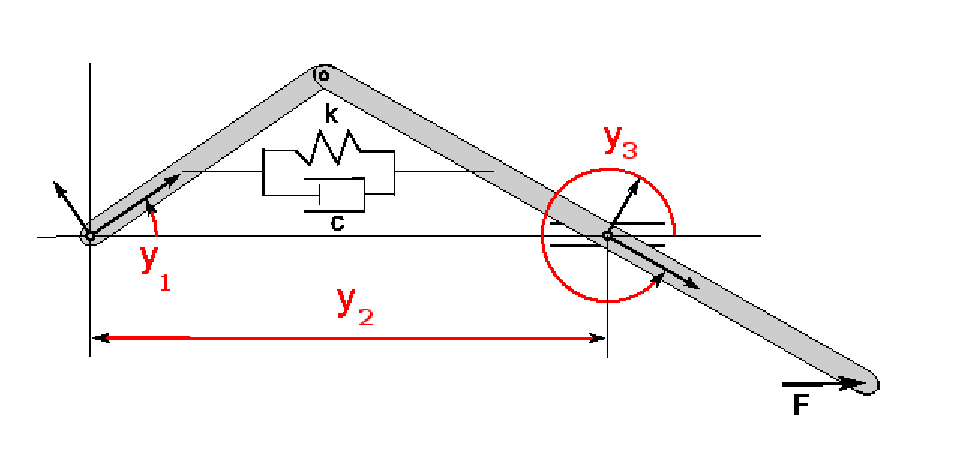
\epsfig{file=figs_slcrank/slider_crank.eps,width=\textwidth}}}
  \caption{Slider-crank mechanism modeled with three generalized coordinates.}
  \label{f:sl_crank}
\end{figure}
%%

The equations of motion can be written as
\begin{equation*}
  \begin{split}
    M(y) \ddot y &= Q(y,\dot y) - \Phi_y^T(y) \lambda \\
    \Phi(y)     &= 0 ~,
  \end{split}
\end{equation*}
where $y \in R^3$ is the vector of generalized coordinates, $M(y)$ is the generalized mass
matrix, and $Q$ is a vector of generalized applied forces. $\Phi(y) \in R^2$ represents the
(algebraic) position-level constraints and $\Phi_y$ is its Jacobian with respect to $y$.
$\lambda \in R^2$ are Lagrange multipliers corresponding to the constraint forces.
%%
For its solution with {\idas}, the above index-3 DAE is reformulated as a stabilized 
index-2 DAE (Gear-Gupta-Leimkuhler formulation, \cite{GGL:85}) by introducing two
additional Lagrange multipliers $\mu$ and appending the velocity constraints.
Converting to first order differential equations, we obtain:
\begin{equation}\label{e:GGLform}
\begin{split}
  \dot y &= v - \Phi_y^T(y) \mu  \\
  M(y) \dot v &= Q(y,v) - \Phi_y^T(y) \lambda \\
  \Phi(y)     &= 0 \\
  \Phi_y(y) v &= 0 ~,
\end{split}
\end{equation}
where $v = \dot y$ are the generalized velocities.

For the mechanical system under consideration, the position constraints can be written as
\begin{equation*}
  \Phi(y) = \begin{bmatrix}
    y_2 - a \cos(y_1) - a \cos(y_3) \\
    a \sin(y_1) + \sin(y_3)
  \end{bmatrix}
\end{equation*}
while the generalized force takes the form
%%
\begin{equation*}
  Q(y, v) = \begin{bmatrix}
    - (f/\ell) a [\sin(y_3-y_1)/2 + y_2 \sin(y_1)]/2 \\
    (f/\ell) [\cos(y_3)/2 - y_2 + a \cos(y_1)/2 ] + F \\
    - (f/\ell) [ y_2 \sin(y_3) - a \sin(y_3-y_1)/2]/2 - F \sin(y_3)
  \end{bmatrix} ~,
\end{equation*}
where
\begin{equation*}
  \begin{split}
    f = & k (\ell - \ell_0) + c {\ell}' \\
    \ell^2 = & y_2^2 - y_2 [\cos(y_3) + a \cos(y_1)] + (1 + a^2)/4 + a \cos(y_3-y_1)/2 \\
    2 \ell {\ell}' = & 2 y_2 v_2 - v_2 [\cos(y_3) + a \cos(y_1)] + y_2 [\sin(y_3)v_3 + a\sin(y_1)v_1] \\
    & - a \sin(y_3-y_1) (v_3-v_1)/2 ~.
  \end{split}
\end{equation*}
The generalized mass matrix is diagonal: $M = diag \{J_1, m_2, J_2\}$.

In the case treated here, $a = .5$, $J_1 = 1$, $J_2 = 2$, $m_1 = m_2 = 1$,
$F = 1$, $k = 1$, $c = 1$, and $\ell_0 = 1$. The final time is $t_f = 10$.

The system (\ref{e:GGLform}) is solved with {\idas} using a state vector
$Y = [y, v, \lambda, \mu] \in R^{10}$.   The initial conditions (at $t = 0$)
are set to consistent values, given as follows:
\begin{equation*}
  \begin{split}
    &y_1 = \pi/2 \\
    &y_3 = \arcsin(-a) \\
    &y_2 = \cos(y_3) \\
    &v_1 = v_2 = v_3 = 0 \\
    &\lambda_1 = \lambda_2 = \mu_1 = \mu_2 = 0 \\
    &dy_1/dt = dy_2/dt = dy_3/dt = 0 \\
    &dv_1/dt = \left[Q_1\right]_{t=0} / J_1 \\
    &dv_2/dt = \left[Q_2\right]_{t=0} / m_2 \\
    &dv_3/dt = \left[Q_3\right]_{t=0} / J_2 \\
    &d\lambda_1/dt = d\lambda_2/dt = d\mu_1/dt = d\mu_2/dt = 0 ~.
  \end{split}
\end{equation*}
The problem is solved with a relative tolerance of $10^{-6}$ and a (scalar) absolute
tolerance of $10^{-7}$. Note that the algebraic variables $\lambda$ and $\mu$ are
excluded from the error test (by specifying them through \id{IDASetId} and invoking
\id{IDASetSuppressAlg}).

The two parameters of the TSD, $k$ and $c$, are considered in a forward
sensitivity analysis of this model. Solution sensitivities with respect
to those parameters are computed and then used to estimate the gradient
of the integrated kinetic energy of the system,
\begin{equation}
  G = \int_{t_0}^{t_f} \left(    
    \frac{1}{2} J_1 \dot y_1^2 + \frac{1}{2} m_2 \dot y_2^2 + \frac{1}{2} J_2 \dot y_3^2 \right) \, dt \, .
\end{equation}
This is then compared against gradient approximations based on (backward, forward, and central)
finite differences.  The sensitivity residuals are evaluated using the {\idas} internal
finite-difference approximation.  Computation of the gradient of the integral in $G$ takes
advantage of the {\idas} feature for computing sensitivities of pure quadrature equations.

Figure \ref{f:x2sensi} shows the sensitivities of the horizontal position of the
translational joint ($x = y_2$) with respect to the TSD parameters $k$ and $c$,
superimposed over the solution itself.
%%
\begin{figure}[h]
  {\centerline{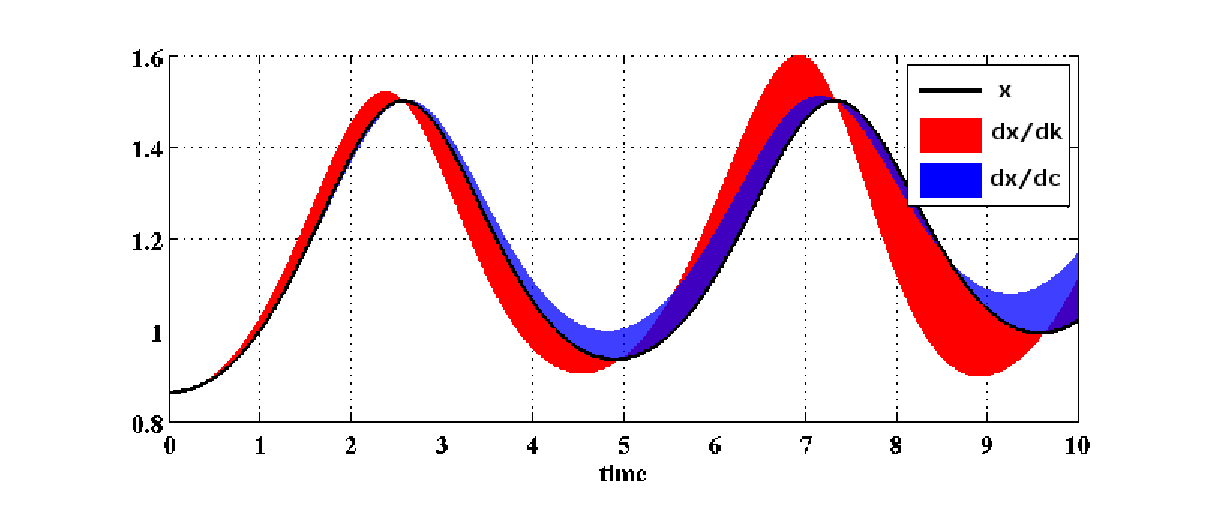
\epsfig{file=figs_slcrank/x2sensi.eps,width=\textwidth}}}
  \caption{Sensitivities of the solution component $y_2$ with respect to the TSD parameters.}
  \label{f:x2sensi}
\end{figure}
%%

The following output is generated by \id{idasSlCrank\_FSA\_dns} when computing
sensitivities with the \id{IDA\_SIMULTANEOUS} method and full error control:

\includeOutput{idasSlCrank\_FSA\_dns}{../../examples/idas/serial/idasSlCrank_FSA_dns.out}


%----------------------------------------------------------------------------------

\subsection{A parallel example using IDABBDPRE: idasBruss\_FSA\_kry\_bbd\_p}
\label{ss:idasBruss_FSA_kry_bbd_p}

The \id{idasBruss\_FSA\_kry\_bbd\_p} program solves the two-species time-dependent
PDE known as the Brusselator problem, using the {\idaspgmr} linear solver and the
{\idabbdpre} preconditioner.

With subscripts on $u$ and $v$ denoting partial derivatives, the PDEs
are as follows:
\begin{equation*}
\begin{split}
  &\partial u / \partial t = \epsilon_1 (u_{xx} + u_{yy})
                              + u^2 v - (B + 1) u + A \\
  &\partial v / \partial t = \epsilon_2 (v_{xx} + v_{yy})
                              - u^2 v + B  u
\end{split}
\end{equation*}
on the unit square in $(x,y)$, and for $0 \leq t \leq t_f = 1$.
The constants involved are $\epsilon_1 = \epsilon_2 = 0.002$, $A = 1$,
and $B = 3.4$.  The boundary conditions are Neumann (zero derivatives).
The initial conditions are given by:
\begin{equation*}
\begin{split}
  &u = 1 - 0.5 \cos(\pi y) \\
  &v = 3.5 - 2.5 \cos(\pi x)
\end{split}
\end{equation*}

The PDEs are discretized by central differencing on a uniform 2D spatial mesh.
The boundary conditions are handled by copying values from the first interior
mesh line to a line of ghost values on each side of the square.
The system is actually implemented on submeshes, processor by processor.

Here the forward sensitivity capability in {\idas} is used to compute
solution sensitivities with respect the two parameters $\epsilon_i$.
From those, we compute the corresponding sensitivities of the final spatial
average of $u$,
\begin{equation*}
  g = \int \int u(x,y,t_f) ~dx~dy
\end{equation*}
by means of a spatial integration of the sensitivities:
\begin{equation*}
  dg/d\epsilon_i = \int \int \partial u(x,y,t_f) / \partial \epsilon_i~dx~dy ~.
\end{equation*}


The following output is generated by \id{idasBruss\_FSA\_kry\_bbd\_p} when computing
sensitivities with the \id{IDA\_SIMULTANEOUS} method and full error control:

\id{mpirun -np 4 idasBruss\_FSA\_kry\_bbd\_p -sensi sim t}

\includeOutput{idasBruss\_FSA\_kry\_bbd\_p}{../../examples/idas/parallel/idasBruss_FSA_kry_bbd_p.out}
